
\section{Recuperação de chaves com erros em criptosistemas baseados no (EC)DLP}

%Due to noise, data leakage (note that we are aiming at exploiting the address leakage only), and other aspects that interfere with the side-channel analysis (misalignment, clock jitter, etc), the derivation of the final scalar for a single trace likely contains errors. 
%
Devido ao ruído, vazamento de dado (por canal lateral) não relacionado à chave secreta, e outros aspectos que interferem com a análise por canal lateral (p.ex., desalinhamento, clock jitter), o escalar final obtido por ataque SCA realizado a partir de um único trace provavelmente conterá erros, isto é, o valor de alguns dos bits recuperados estará incorreto.

%
%If the amount of wrong bits is sufficiently small, then a brute-force attack may still be feasible. 
%
Se a quantidade de bits incorretos (erros) é suficientemente pequena, então um ataque de força bruta pode ser viável, mesmo que não se saiba a localização de tais bits incorretos. A complexidade de tal busca, isto é, o número de escalares que devem ser testados até o escalar correto ser encontrado é ${{n}\choose{s}} 2^s$, onde $n$ é o comprimento do escalar em bits e $s$ é número de erros. Considerando um escalar de $n = 256$ bits\footnote{comprimento típico do escalar para uma curva no nível de segurança de 128 bits}, o valor máximo de $s$ para concluir tal busca em tempo aceitável é 6, o que significa que aproximadamente $2^{56}$ escalares precisam ser testados.

%
% However, first the attacker needs a metric to indicate the location of the possible wrong bits in the recovered scalar. 
%
Se a quantidade de bits incorretos for maior, então o atacante necessita saber a localização dos possíveis bits incorretos nos escalar recuperado para corrigi-los em tempo viável.
%
% The notion of suspicious bits (cf.~\Cref{cswap-arith-template-gen-and-match}) can be used as a reference for the scalar bits selection with respect to a brute-force attack. 
%
Neste caso, a noção de bits suspeitos\erick{definir} pode ser usada como referência para a seleção de bits do escalar com respeito a um ataque de força bruta. 
%

\newcommand{\scalarlen}{254}

% Let us consider the trace with smallest amount of suspicious bits from the experiment from (Section\erick{ref. Section load attack SAC2016}} as an example; for this trace there are $\iterations$ suspicious bits that comprise all falsely identified bits.
%%%
Vamos supor que para um dado trace o escalar recuperado tem $s=54$ bits suspeitos, de um total de $\scalarlen$ bits.
%%%
% Unfortunately, to recover a full randomized scalar, even in this case, the attacker needs $O(2^{\iterations})$ operations, which is generally impractical. % Note, that we consider only the worst-case complexity and not the average case. 
%%%
Infelizmente, para recuperar tal escalar, se este foi completamente aleatorizado pela contramedida SR, o atacante precisa realizar $O(2^{\scalarlen})$ operações, no pior caso, o que geralmente não é prático.\footnote{Nesta subseção são consideradas apenas complexidades de pior caso.}


%%%
% To improve the brute-force complexity, there are two options.
%%%
Para melhorar esta complexidade de força bruta, há duas opções.
%%%
% The first approach is to try to exploit the distribution of suspicious bits for incorrectly (red) and correctly (blue) recovered bits (\Cref{fig:hist-conf-all-traces__n_trset_40}). While there is a clear trend for incorrect bits to have lower confidence score, the intersection between correct and incorrect bits is large. 
%%%
A primeira abordagem é tentar explorar a distribuição dos bits suspeitos nos conjuntos de bits recuperados incorretamente e corretamente (\Cref{fig:hist-conf-all-traces__n_trset_40}). Enquanto há uma clara tendência dos bits incorretos terem um confidence score menor, a área da intersecção entre as duas distribuições é grande.
%%%
% Still, it may possible to exploit the trend with an informed brute force attack~\cite{kang2014}, prioritizing bits with the lowest confidence score.
%%%
Ainda assim, pode ser possível explorar esta tendência com um ataque de força bruta informado~\cite{LangeVredendaalWakker2014}, priorizando os bits com os menores confidence scores.
%%%
% Unfortunately this attack works well if the bits containing errors are adjacent and that is not the case in our setting. 
%%%
Infelizmente esse ataque funciona bem se os bits contendo erros são adjacentes e este não é o caso no nosso contexto.
%%%

\begin{figure}[h!tb]
	\centering   %height=0.20\textheight
	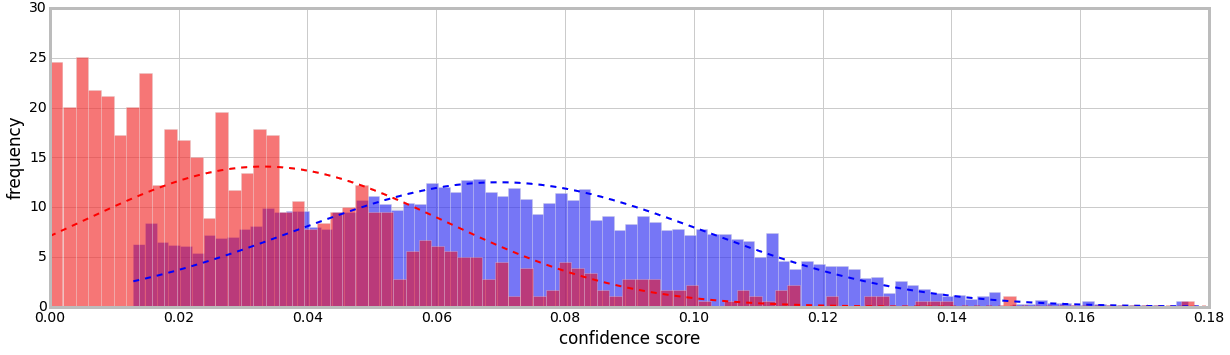
\includegraphics[width=0.9\textwidth]{figures/SAC_2016__pointer_cswap_attack__hist-conf-all-traces__n_trset_40.png}
	\caption{
	%Distribution of confidence scores over all traces for suspicious bits. Red: incorrectly recovered bits, blue: correctly recovered but suspicious bits.
	Distribuição de confidence scores de bits suspeitos para um conjunto de $1000$ traces de execuções completas da ECSM. Vermelho: bits recuperados incorretamente; azul: bits corretamente recuperados porém considerados suspeitos.
	}
	\vspace{.5mm}
	\label{fig:hist-conf-all-traces__n_trset_40}
\end{figure}

\subsection{Algoritmo de Gopalakrishnan, Theriault e Yao~\cite{GopalakrishnanTheriaultYao07}} %\erick[inline]{copiar texto do paper SAC. Baseado no paradigma time-memory trade-off}

% Alternatively (or combined with the informed brute-force search), we apply the second algorithm from~\cite{chain_recovery_2007}, which is originally designed for \emph{square-and-multiply chains}, to the Montgomery ladder. 
%%%
Alternativamente, ou combinado com uma busca de força bruta informada, nós aplicamos o segundo algoritmo de~\cite{Gopalakrishnan2007} à Montgomery ladder. Tal algoritmo é baseado no compromisso entre tempo e memória (\textit{time-memory trade-off}) e foi originalmente projetado para~\textit{cadeias de quadrado e multiplicação}.


%%%
% We describe how the algorithm works using the aforementioned example trace,  which contains $s=\iterations$ suspicious bits, as an example. Let us represent the indices of these bits as a list sorted in descending order: $i_s, \dots i_1$, 
%%%
Nós descrevemos como o algoritmo funciona tomando como um exemplo um escalar recuperado contendo $s=54$ bits suspeitos. Vamos representar os índices deste bits como uma lista ordenada em ordem decrescente: $i_s, \dots i_1$,
%%%
% where each $i_j \in \{0, \dots 254\}$ and $s \ge j \ge 1$; note that there are $255$~bits in total. Let $x$ denote the bit index $i_{\floor*{\frac{s}{2} + 1}}$ (namely, $i_{\x}$ for the example trace). 
%%%
onde cada $i_j \in \{0, \dots 254\}$ e $s \ge j \ge 1$; note que há $255$~bits no total. Seja $x$ o índice $i_{\floor*{\frac{s}{2} + 1}}$.
%%%
%Let $a$ be the number represented by the bit string corresponding to the left part of the scalar from $x$ (including $i_x$) and let $b$ be the number corresponding to the bit string of the (least significant) right part.
%%%
Seja $a$ o número representado pela string de bits correspondente a parte esquerda do escalar (mais significativa) antes de $x$ (incluindo $i_x$) e seja $b$ o número correspondente à string de bits da parte direita (menos significativa).
%%%
%let $y=254-i_x$ be the length of the right part. Furthermore, we know that $R = [k] P$, 
%%%
Seja $y=254-i_x$ o comprimento da parte direita. Além disso, sabemos que $R = [k] P$,
%%%
%where $R$ is the resulting point, $k$ the scalar to be recovered, 
% and $P$ the input point. 
%%%
onde $R$ é o ponto resultante, $k$ é o escalar correto a ser recuperado e $P$ é o ponto de entrada.
%%%


% Then, clearly 
%\begin{equation*}
% $R = [k] P = [a \cdot 2^{i_x} + b] P = [a] ([2^{i_x}] P) + [b] P$. 
%\end{equation*}
%%%
Então, claramente $R = [k] P = [a \cdot 2^{i_x} + b] P = [a] ([2^{i_x}] P) + [b] P$. 
%%%
% If we denote $[2^{i_x}] P$ by $H$, then the above equation reduces to
% \begin{equation}\label{eq:check}
% R - [b] P = [a] H
% \end{equation}
%%%
Se nós denotamos $[2^{i_x}] P$ por $H$, então a equação acima se reduz a
\begin{equation}\label{eq:check}
R - [b] P = [a] H
\end{equation}
%%%


%We can use Equation~\ref{eq:check} to check correctness of our guess. 
%Now, following~\cite{chain_recovery_2007}, we use a time-memory trade-off technique to speed up an exhaustive search: 
%Consider all different possible guesses for $a$. 
%%%
Nós podemos usar \erick{CONT HERE}.
%TODO
%%%
%For each guess, we compute $[a] H$ and store all pairs $(a, [a] H)$. 
%We then sort all pairs based on the value of $[a] H$ and store them in an ordered table.
%%%
%TODO
%%%



% Next, we make a guess for $b$ and compute $z = R - [b] P$. 
%If our guess for $b$ 
%is correct, then $z$ is present in the second column of some row in the table we built---the first column is the corresponding $a$. 
%Finding such a pair can be done using binary search, as the table is sorted as per the second column. 
%%%
%TODO
%%%
%If $z$ is present, we are done since we have determined the scalar. 
%Otherwise, we make a new, different guess for $b$ and continue. 
%%%
%TODO
%%%
%Since there are approximately $2^{\frac{s}{2}}$ guesses for $a$ and $b$, the time complexity is $O(2^{\frac{s}{2}})$ operations. 
% As there are $2^{\frac{s}{2}}$ guesses for $a$, the table has that many entries and the space complexity is $O(2^{\frac{s}{2}})$ points.
%%%
%TODO
%%%
% This way, we limit the time complexity to $O(2^{\frac{s}{2}})$ (cf.~\cite{chain_recovery_2007} for a detailed complexity analysis), which is $O(2^{\complexity})$ for the example trace. 
%%%
%TODO
%%%



% We do not know which trace contains the smallest number of suspicious bits since we do not know the maximum confidence score of a falsely identified bit. 
% However, to use the above algorithm we assume that we know the number of suspicious bits to be bruteforced to recover the correct scalar. 
%%%
%TODO
%%%
% This can be determined by using templates to attack some traces, for which we know the randomized key. 
% Furthermore, note that if the attack fails, we can extend the execution to the second most likely suspicious bit and reuse the previously obtained data. 
%%%
%TODO
%%%
% Based on our experiments, we determined that the number $54$ of suspicious bits should cover all falsely identified bits for at least one trace. 
% Our complete attack works as follows: in parallel, we run the above algorithm for each of the $n$ traces. 
% We stop the attack as soon as the time-memory trade-off technique succeeds for one trace. 
%%%
%TODO
%%%



% Since we are running the attack $n$ times in parallel the complexity of the complete attack is multiplied by $n$. 
%The complexity totals $O(n \cdot 2^{\frac{s}{2}})$ operations and $O(n \cdot 2^{\frac{s}{2}})$ points in memory. 
%%%
%TODO
%%%
% For the attack from the previous section, this corresponds to $O\left(\n \cdot 2^{\complexity}\right) = O\left(2^{\total}\right)$ operations. 
%%%
%TODO
%%%
% Therefore, We conclude that we can efficiently recover the scalar successfully even in the presence of multiple errors and uncertain bits (for experimental results see~\cref{recovery_experimental}). 
%%%
%TODO
%%%
% Furthermore, we believe that the above technique may be of independent interest since it can be applied to a commonly used ECSM algorithm, i.e., Montgomery ladder, even if errors are spread independently in the scalar.
%%%
%TODO
%%%


\subsection{Aplicação do Algoritmo de Gopalakrishnan, Theriault e Yao~\cite{GopalakrishnanTheriaultYao07} à curva elíptica Curve25519}

\erick[inline]{Explicar as otimizações de desempenho que podem ser aplicadas à nível de aritmética na curva}

\begin{comment}
The first challenge we faced is how to compute the point subtraction in Equation 2. Curve25519 is a curve in the Montgomery form, and as such, there is an efficient formula for differential point addition using XZ coordinates, but no efficient formula to compute a standard point addition, as far as we know. For that reason, we decided to do the point addition in affine coordinates, which costs a field inversion and a few multiplications. However, to use them we need to know the $y$-coordinates $y(R)$ and $y([b]P)$. The attack assumes that $x(R)$ (the ECSM output) is known, but $y(R)$ is not, and thus has to be computed. To do so, we use the curve formula directly to compute the two possible values for $y(R)$, at the cost of a field square root, an expensive operation, but it has to be done only once for each value of $R$. In the case of $y([b]P)$, an efficient algorithm by Okeya and Sakurai~\cite{OkeyaSakurai2001} costs one field inversion.

To generate the table of precomputed points $A = [a]H$ and to compute $B = [b]P$ in~\cref{eq:check}, the naive approach is to compute a full ECSM for each value of $a$ and $b$. A more efficient method is to apply Gray coding to the suspicious bits in scalars $a$ and $b$. One property of such a code is that consecutive code words differ in just a single bit, which means that, in our context, we can generate $[k']P$ from $[k]P$ using a single point addition (if the bit changed from 0 to 1) or point subtraction (if the change is from 1 to 0), where $k$ and $k'$ are scalars whose unknown bits are represented as Gray code words, and the code word in $k'$ is the successor of the respective code word in $k$. To compute the sequence of points $[k_i]P$ ($i=0,1...$), we first construct the scalar $k_0$, by setting the unknown bits to zero and the (assumed correct) recovered bits from the output of the SCA attack to their respective values. Then, we apply the full ECSM algorithm to compute $[k_0]P$, and from there we use the aforementioned method to generate the sequence of points $[k_1]P, [k_2]P \dots$, which costs essentially a point addition per each computed point.

We implemented the key recovery algorithm with the aforementioned arithmetic-level optimizations as a single-threaded program. We tested our implementation in a smaller scale, to recover 40 suspicious bits of a scalar on a PC with 8GB of RAM total, but only 5GB available for the program, a i7-3740QM CPU, running at 2.7GHz. It took 1h23 to recover the correct scalar, where about 1.5ms is spent to add a single entry to the table and about 3ms 
%is spent 
to test a possible value of b. By using these time values as a reference, we estimate that the time for the recovery of a scalar with 60 suspicious bits using the current implementation is around 18 days. The source code of the key recovery implementation is publicly available~\cite{source-repo-keyrecovery}.
\end{comment}


\begin{comment}
%\subsection{Algoritmo de Lange, Vrendendaal e Wakker~\cite{LangeVredendaalWakker2014}}
%\erick[inline]{baseado no algoritmo de Pollard-Kangaroo. Utilizar texto da discussão por email com os autores.}
\end{comment}